\documentclass[MASTER.tex]{subfiles} 
\begin{document} 
\begin{frame}
		\frametitle{Classification with \texttt{scikit.learn}}
		\Large
\noindent \textbf{Classification with scikit-learn}
\begin{itemize}
\item Here we look at problem of classification, a situation in which a response is a categorical variable. 
\item We will build upon the techniques that we previously discussed in the context of regression and show how they can be transferred to classification problems. 
\item Here we will introduce a number of classification techniques, and it will try to convey their corresponding strengths and weaknesses by visually inspecting the decision boundaries for each model.
\end{itemize}

\end{frame}
%===========================================================%
\begin{frame}
	\frametitle{Classification with \texttt{scikit.learn}}
	\Large
	\begin{itemize}
%	\item This is part of a series of blog posts showing how to do common statistical learning techniques with Python. 
	\item We provide only a small amount of background on the concepts and techniques we cover, so if you’d like a more thorough explanation check out Introduction to Statistical Learning or sign up for the free online course run by the book’s authors here.
	\end{itemize}

\end{frame}
%===========================================================%
%\begin{frame}	\frametitle{Classification with \texttt{scikit.learn}}
%	\Large
%\textbf{Scikit-learn}\\
%In this post we will use \textbf{scikit-learn}, an easy-to-use, general-purpose toolbox for machine learning in Python. We will use it extensively in the coming posts in this series so it’s worth spending some time to introduce it thoroughly.
%\end{frame}
%===========================================================%
\begin{frame}
	\Large
\noindent	\textbf{Scikit-learn}\\
	\begin{itemize}
	\item Scikit-learn is a library that provides a variety of both supervised and unsupervised machine learning techniques. 
	\item Supervised machine learning refers to the problem of inferring a function from labeled training data, and it comprises both regression and classification. 
	\end{itemize}


\end{frame}
%===========================================================%
\begin{frame}
	\Large
	
\noindent \textbf{Unspervised Learning}
	\begin{itemize}
		\item	
	Unsupervised machine learning, on the other hand, refers to the problem of finding interesting patterns or structure in the data; it comprises techniques such as clustering and dimensionality reduction.
	\item  In addition to statistical learning techniques, scikit-learn provides utilities for common tasks such as model selection, feature extraction, and feature selection.
\end{itemize}
\end{frame}
%===========================================================%
\begin{frame}[fragile]
	\Large
\noindent	\textbf{Estimators}
\begin{itemize}
\item Scikit-learn provides an object-oriented interface centered around the concept of an Estimator. \item According to the scikit-learn tutorial “\textit{An estimator is any object that learns from data; it may be a classification, regression or clustering algorithm or a transformer that extracts/filters useful features from raw data.}” 	
\end{itemize}
\end{frame}


%===========================================================%
\begin{frame}[fragile]
	\Large
\begin{itemize}
\item The \texttt{Estimator.fit} method sets the state of the estimator based on the training data. 
\item Usually, the data is comprised of a two-dimensional numpy array X of shape \texttt{(n\_samples, n\_predictors) }that holds the so-called feature matrix and a one-dimensional numpy array y that holds the responses. 
\item Some estimators allow the user to control the fitting behavior. 
\end{itemize}
\end{frame}


%===========================================================%
\begin{frame}[fragile]
	\Large
	\begin{itemize}
		\item For example, the \texttt{sklearn.linear\_model.LinearRegression} estimator allows the user to specify whether or not to fit an intercept term. 
\item This is done by setting the corresponding constructor arguments of the estimator object:
\end{itemize}
\end{frame}
%===========================================================%
\begin{frame}[fragile]
	\begin{figure}
\centering
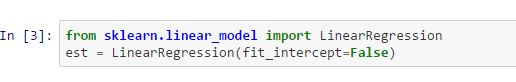
\includegraphics[width=1.1\linewidth]{sklcass/sklclass1a}

\end{figure}

\large
\begin{framed}
\begin{verbatim}
from sklearn.linear_model import LinearRegression
est = LinearRegression(fit_intercept=False)
\end{verbatim}
\end{framed}

%The docstring of the estimator shows you all available arguments – in IPython simply use LinearRegression? to view the docstring.
\end{frame}
%===========================================================%
\begin{frame}[fragile]
\Large
\begin{itemize}
\item During the fitting process, the state of the estimator is stored in instance attributes that have a trailing underscore ('\_'). 
\item For example, the coefficients of a LinearRegression estimator are stored in the attribute \texttt{coef\_}:
\end{itemize}

\end{frame}
%===========================================================%
\begin{frame}[fragile]
\begin{framed}
\begin{verbatim}
import numpy as np

# random training data
X = np.random.rand(10, 2)
y = np.random.randint(2, size=10)
est.fit(X, y)
est.coef_   # access coefficients

# Output : array([ 0.33176871,  0.34910639])
\end{verbatim}
\end{framed}
\end{frame}
%===========================================================%
\begin{frame}[fragile]
	\textbf{Estimators}
\Large
\begin{itemize}
\item Estimators that can generate predictions provide a Estimator.predict method.
\item In the case of regression, Estimator.predict will return the predicted regression values; it will return the corresponding class labels in the case of classification.
\item  Classifiers that can predict the probability of class membership have a method \texttt{Estimator.predict\_proba} that returns a two-dimensional numpy array of shape \texttt{(n\_samples, n\_classes)} where the classes are lexicographically ordered.
\end{itemize}

\end{frame}

%%===========================================================%
%\begin{frame}[fragile]
%\textbf{Estimators: Transformers}
%\begin{itemize}
%\item Finally, there is a special type of Estimator called Transformer which transforms the input data — e.g. selects a subset of the features or extracts new features based on the original ones.
%%\item In addition to a fit method, a Transformer object provides the following methods:
%\end{itemize}
%
%\end{frame}

%%===========================================================%
%\begin{frame}[fragile]
%\Large
%\begin{framed}
%	\begin{verbatim}
%class Transformer(Estimator):
%
%def transform(self, X):
%"""Transforms the input data. """
%# transform ``X`` to ``X_prime``
%return X_prime
%\end{verbatim}
%\end{framed}
%\end{frame}
%%===========================================================%
%\begin{frame}[fragile]
%	\begin{itemize}
%	\item Usually, a Transformer does not provide a predict method, but in some cases it may.
%	\item One transformer that we will use in this posting is \texttt{sklearn.preprocessing.StandardScaler}. 
%	\item This transformer centers each predictor in X to have zero mean and unit variance:
%	\end{itemize}
%
%\end{frame}
%===========================================================%
%\begin{frame}[fragile]
%In [6]:
%from sklearn.preprocessing import StandardScaler
%scaler = StandardScaler(copy=True)  # always copy input data (don't modify in-place)
%X_centered = scaler.fit(X).transform(X)
%scaler.mean_  # mean that will be subtracted upon transform
%Out[6]:
%array([ 0.48261456,  0.48636312])
%For more information on scikit-learn please consult the detailed user guide or walk through the excellent tutorial.
%\end{frame}
\begin{frame}
	\huge
\[ \mbox{ Classification with Scikit-Learn} \]
\end{frame}
%===========================================================%
\begin{frame}[fragile]
\textbf{Understanding Classification}\\
Although regression and classification appear to be very different they are in fact similar problems.

\begin{itemize}
\item In regression our predictions for the response are real-valued numbers
\item on the other hand, in classification the response is a mutually exclusive class label 
\item Example ``\textit{Is the email spam?}" or ``\textit{Is the credit card transaction fraudulent?}".
\end{itemize}

\end{frame}
%===========================================================%
\begin{frame}[fragile]

 	\Large
 	\textbf{Binary Classsification Problems}\\
 	\begin{itemize}
\item If the number of classes is equal to two, then we call it a binary classification problem; if there are more than two classes, then we call it a multiclass classification problem.
\item  In the following we will assume binary classification because it’s the more general case, and — we can always represent a multiclass problem as a sequence of binary classification problems.
\end{itemize}

\end{frame}
%===========================================================%
\begin{frame}[fragile]
	\Large
\textbf{Credit Card Fraud}
\begin{itemize}
\item We can also think of classification as a function estimation problem where the function that we want to estimate separates the two classes. 
\item This is illustrated in the example below where our goal is to predict whether or not a credit card transaction is fraudulent
\item he dataset is provided by James et al., \textbf{Introduction to Statistical Learning}.
\end{itemize}

\end{frame}

%===========================================================%
\begin{frame}[fragile]
	\Large
\vspace{-1cm}
\textbf{Credit Card Fraud}
\begin{figure}
\centering
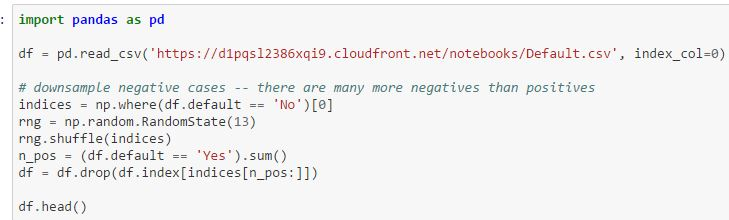
\includegraphics[width=1.2\linewidth]{sklcass/sklclass1}

\end{figure}

\end{frame}
%===========================================================%
\begin{frame}[fragile]
	\Large
\textbf{Credit Card Fraud}
\begin{figure}
\centering
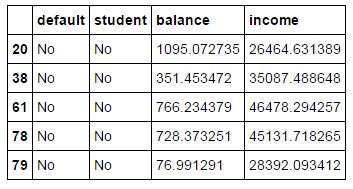
\includegraphics[width=0.7\linewidth]{sklcass/sklclass2}

\end{figure}

\end{frame}

%===========================================================%
\begin{frame}[fragile]
	\Large
	\textbf{Credit Card Fraud}
	\begin{itemize}
\item 	On the left you can see a scatter plot where fraudulent cases are red dots and non-fraudulent cases are blue dots. 
\item A good separation seems to be a vertical line at around a balance of 1400 as indicated by the boxplots on the next slide.
	\end{itemize}
	

\end{frame}

%===========================================================%
\begin{frame}[fragile]
	
	\begin{figure}
\centering
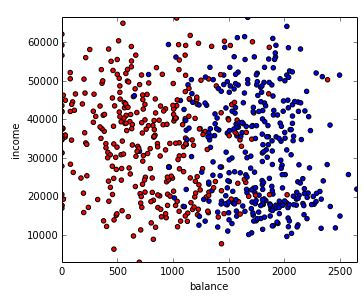
\includegraphics[width=0.95\linewidth]{sklcass/sklclass3}

\end{figure}

	
\end{frame}

%======================================================%
\begin{frame}
\begin{figure}
\centering
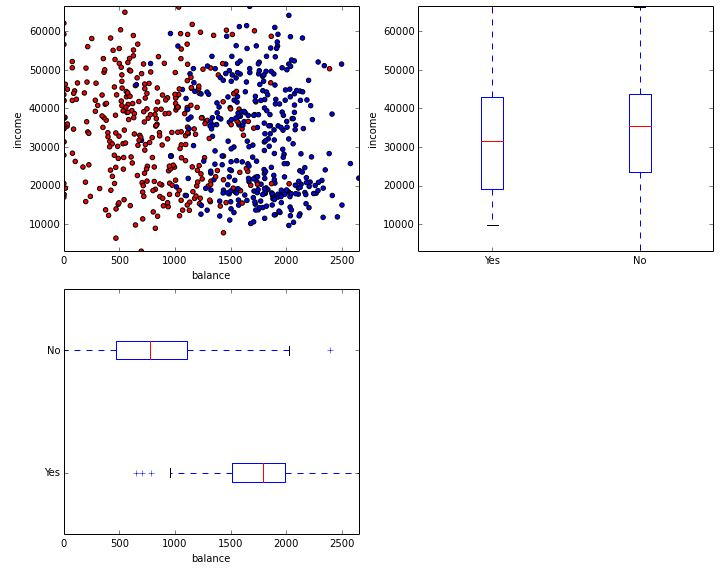
\includegraphics[width=0.9\linewidth]{sklcass/sklclass4}

\end{figure}
\end{frame}
%======================================================%
\begin{frame}
	
	\Large
\textbf{Simple Approach - Linear Regression}
\begin{itemize}
\item A simple approach to binary classification is to simply encode default as a numeric variable with 'Yes' == 1 and 'No' == -1; fit an Ordinary Least Squares regression model and use this model to predict the response as 'Yes' if the regressed value is higher than 0.0 and 'No' otherwise. 
\item The points for which the regression model predicts 0.0 lie on the so-called decision surface — since we are using a linear regression model, the decision surface is linear as well.
\end{itemize}

\end{frame}

%======================================================%
%\begin{frame}
%The example below illustrates this. Note that we use the \texttt{sklearn.linear\_model.LinearRegression} class in scikit-learn instead of the statsmodels.api.OLS class in statsmodels – they both implement the same procedure.
%\end{frame}
%======================================================%
\begin{frame}
\begin{figure}
\centering
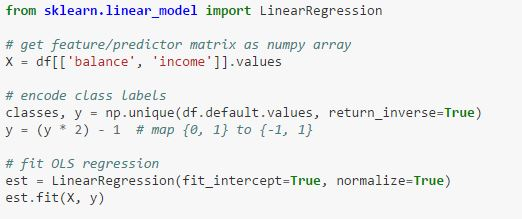
\includegraphics[width=0.99\linewidth]{sklcass/sklclass6}
\end{figure}

\end{frame}
%======================================================%
\begin{frame}
\begin{figure}
\centering
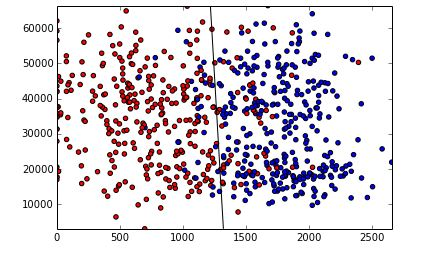
\includegraphics[width=0.99\linewidth]{sklcass/sklclass7}

\end{figure}

\end{frame}
%======================================================%
\begin{frame}
	\begin{itemize}
	\item Points that lie on the left side of the decision boundary will be classified as negative; 
	\item Points that lie on the right side, positive. 
	\end{itemize}

%The implementation of plot_surface can be found in the Appendix. 
\end{frame}

%======================================================%
\begin{frame}
	\Large
\textbf{Confusion Matrix}
\begin{itemize}
\item We can assess the performance of the model by looking at the confusion matrix — a cross tabulation of the actual and the predicted class labels. 

\item The correct classifications are shown in the diagonal of the confusion matrix. The off-diagonal terms show you the \textbf{classification errors}. 
\item A condensed summary of the model performance is given by the \textbf{misclassification rate} determined simply by dividing the number of errors by the total number of cases.
\end{itemize}

\end{frame}

%======================================================%
\begin{frame}
\textbf{Confusion Matrix}\begin{figure}
\centering
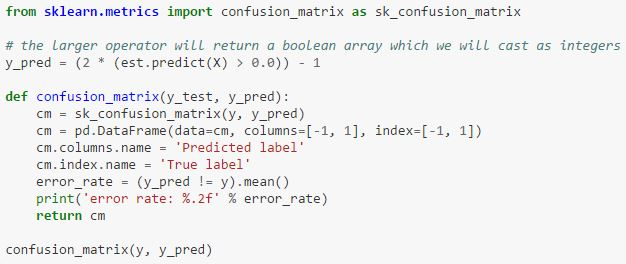
\includegraphics[width=0.95\linewidth]{sklcass/sklclass8}

\end{figure}
\end{frame}
%======================================================%
\begin{frame}
\textbf{Confusion Matrix}
\begin{figure}
\centering
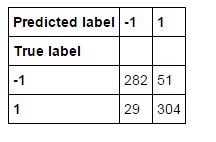
\includegraphics[width=0.7\linewidth]{sklcass/sklclass9}

\end{figure}


\end{frame}
%======================================================%
\begin{frame}
	\large
	\textbf{Cross Validation}
\begin{itemize}
\item In this example we are assessing the model performance on the same data that we used to fit the model. 
\item This might be a biased estimate of the models performance, for a classifier that simply memorizes the training data has zero training error but would be totally useless to make predictions.
\item  It is much better to assess the model performance on a separate dataset called the test data.
\item  Scikit-learn provides a number of ways to compute such held-out estimates of the model performance. \item One way is to simply split the data into a \textbf{training set} and \textbf{testing set}.
\end{itemize}

\end{frame}
%======================================================%
\begin{frame}
\begin{figure}
\centering
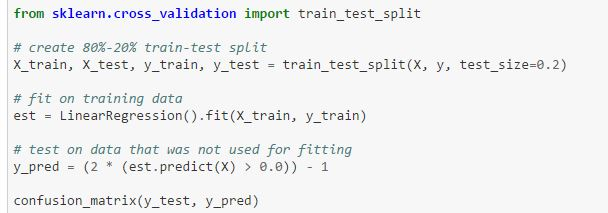
\includegraphics[width=0.99\linewidth]{sklcass/sklclass10}

\end{figure}

\end{frame}
%======================================================%
\begin{frame}[fragile]
\begin{figure}
\centering
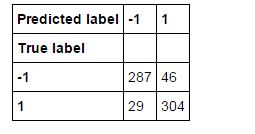
\includegraphics[width=0.7\linewidth]{sklcass/sklclass11}

\end{figure}

\end{frame}
%======================================================%
\begin{frame}[fragile]
\Large
\textbf{Classification Techniques}
\begin{itemize}
\item Different classification techniques can often be compared using the type of decision surface they can learn. \item The decision surfaces describe for what values of the predictors the model changes its predictions and it can take several different shapes: piece-wise constant, linear, quadratic, vornoi tessellation, \ldots
\end{itemize}

\end{frame}
%======================================================%
\begin{frame}[fragile]
\Large
This next part will introduce three popular classification techniques: 
\begin{itemize}
\item[1] Logistic Regression, 
\item[2] Discriminant Analysis, 
\item[3] Nearest Neighbor.
\end{itemize} We will investigate what their strengths and weaknesses are by looking at the decision boundaries they can model. In the following we will use three synthetic datasets that we adopted from this scikit-learn example.
\end{frame}
%======================================================%
\begin{frame}
	\textbf{Synthetic Data Sets}
\begin{figure}
\centering
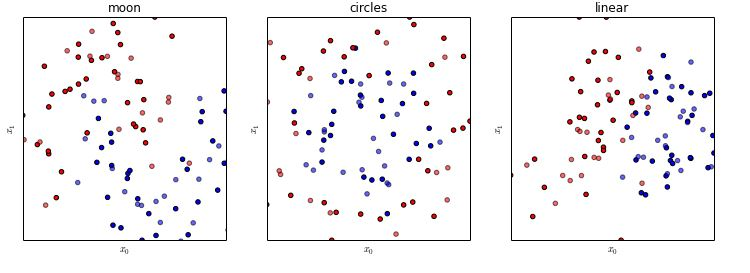
\includegraphics[width=0.99\linewidth]{sklcass/sklclass12}

\end{figure}
\end{frame}
%======================================================%
\begin{frame}
\textbf{Synthetic Data Sets}
\begin{itemize}
\item The task in each of the above examples is to separate the red from the blue points. 
\item Testing data points are plotted in lighter color. 
\item The left example contains two intertwined moon sickles; the middle example is a circle of blues framed by a ring of reds; and the right example shows two linearly separable gaussian blobs.
\end{itemize}

\end{frame}

%======================================================%
\begin{frame}
		\frametitle{Method 1: Logistic Regression}
\textbf{Logistic Regression}
\begin{itemize}
\item Logistic regression can be viewed as an extension of linear regression to classification problems. \item One of the limitations of linear regression is that it cannot provide class probability estimates. 
\item This is often useful, for example, when we want to inspect manually the most fraudulent cases. 
\item Basically, we would like to constrain the predictions of the model to the range $[0,1]$ so that we can interpret them as probability estimates. 
\item In Logistic Regression, we use the logit function to clamp predictions from the range $[−infty,infty]$ to $[0,1]$. 
\end{itemize}

\end{frame}
%======================================================%
\begin{frame}
		\frametitle{Method 1: Logistic Regression}
	\textbf{Logistic Transformation}
	\begin{figure}
\centering
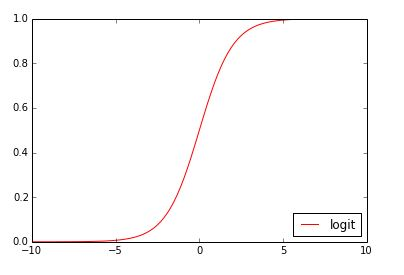
\includegraphics[width=0.7\linewidth]{sklcass/sklclass13}

\end{figure}

\end{frame}
%======================================================%
\begin{frame}
		\frametitle{Method 1: Logistic Regression}
	\Large
	\textbf{Logistic Regression}
\begin{itemize}
\item Logistic regression is available in scikit-learn via the class \texttt{sklearn.linear\_model.LogisticRegression}. 
%\item It uses liblinear, so it can be used for problems involving millions of samples and hundred of thousands of predictors. 
\item Lets see how Logistic Regression does on our three toy datasets.
\end{itemize}

\end{frame}


%======================================================%
\begin{frame}[fragile]
		\frametitle{Method 1: Logistic Regression}
	\begin{framed}
		\begin{verbatim}
from sklearn.linear_model import LogisticRegression

est = LogisticRegression()
plot_datasets(est)
	\end{verbatim}
\end{framed}
\end{frame}

%======================================================%
\begin{frame}
		\frametitle{Method 1: Logistic Regression}
	\begin{figure}
		\centering
		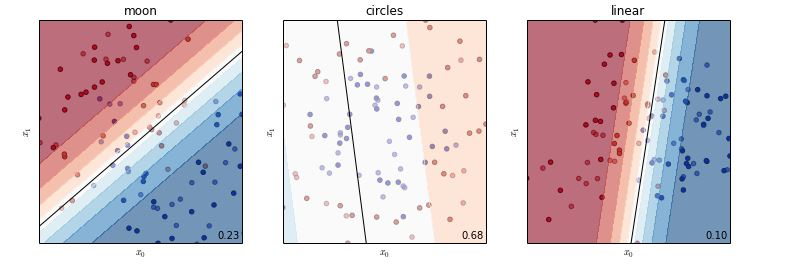
\includegraphics[width=1.1\linewidth]{sklcass/sklclass21}
		
	\end{figure}
\end{frame}
%======================================================%
\begin{frame}
	\frametitle{Method 1: Logistic Regression}
	\Large
	\textbf{Model Appraisal}
\begin{itemize}
\item	As we can see, a linear decision boundary is not a poor approximation for the moon datasets, although we fail to separate the two tips of the sickles in the center. 
\item The cicles dataset, on the other hand, is not well suited for a linear decision boundary. 
\end{itemize}
\end{frame}
%======================================================%
\begin{frame}
	\frametitle{Method 1: Logistic Regression}
		\Large
		\textbf{Model Appraisal}
	\begin{itemize}
		
		\item The error rate of 0.68 is in fact worse than random guessing. \item For the linear dataset we picked in fact the correct model class — the error rate of 10\% is due to the noise component in our data. 
\item The gradient shows you the probability of class membership — white shows you that the model is very uncertain about its prediction.
\end{itemize}

\end{frame}

%======================================================%
\begin{frame}
\frametitle{Method 2: Linear Discriminant Analysis}
\Large
\textbf{Linear Discriminant Analysis}
\begin{itemize}
\item Linear discriminant Analysis (LDA) is another popular technique which shares some similarities with Logistic Regression. 
\item LDA too finds linear boundary between the two classes where points on side are classified as one class and those on the other as classified as the other class.
\end{itemize}

\end{frame}

%======================================================%
\begin{frame}[fragile]
\frametitle{Method 2: Linear Discriminant Analysis}	
\Large
\begin{framed}
\begin{verbatim}

from sklearn.lda import LDA

est = LDA()
plot_datasets(est)
		\end{verbatim}
	\end{framed}
\end{frame}
%%======================================================%
\begin{frame}
\frametitle{Method 2: Linear Discriminant Analysis}
\textbf{Model Appraisal}
\begin{figure}
\centering
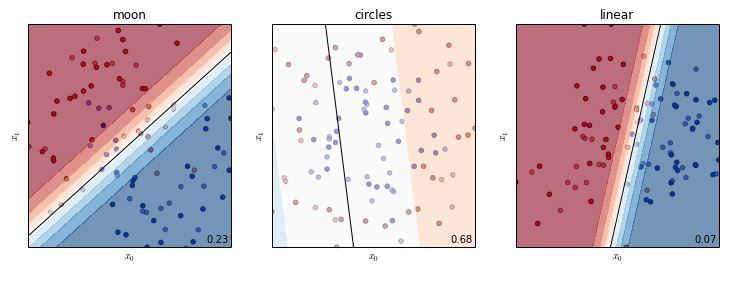
\includegraphics[width=0.95\linewidth]{sklcass/sklclass15}

\end{figure}
(Remark - almost same as logistic regression)
\end{frame}
%======================================================%
\begin{frame}
	\frametitle{Method 2: Linear Discriminant Analysis}
\Large
\textbf{Linear Discriminant Analysis}
\begin{itemize}
\item The major difference between LDA and Logistic Regression is the way both techniques picks the linear decision boundary.
\item  Linear Discriminant Analysis models the decision boundary by making distributional assumptions about the data generating process 
\item Logistic Regression models the probability of a sample being member of a class given its feature values.
\end{itemize}
\end{frame}

%======================================================%
\begin{frame}
	\frametitle{Method 3: Nearest Neighbor}
\Large
\textbf{Nearest Neighbor}
\begin{itemize}
\item Nearest Neighbor uses the notion of similarity to assign class labels; it is based on the smoothness assumption that points which are nearby in input space should have similar outputs.
\item  It does this by specifying a similarity (or distance) metric, and at prediction time it simply searches for the k most similar among the training examples to a given test example.
\end{itemize}
\end{frame}

%======================================================%
\begin{frame}
		\frametitle{Method 3: Nearest Neighbor}
	\Large
	\textbf{Nearest Neighbor}
	\begin{itemize} 
		\item The prediction is then either a majority vote of those k training examples or a vote weighted by similarity. \item The parameter k specifies the smoothness of the decision surface.\item  The decision surface of a k-nearest neighbor classifier can be illustrated by the \textbf{Voronoi tesselation} of the training data, that show you the regions of constant respones.
\end{itemize}
\end{frame}
%======================================================%
\begin{frame}
		\frametitle{Method 3: Nearest Neighbor}
	\begin{figure}
		\centering
		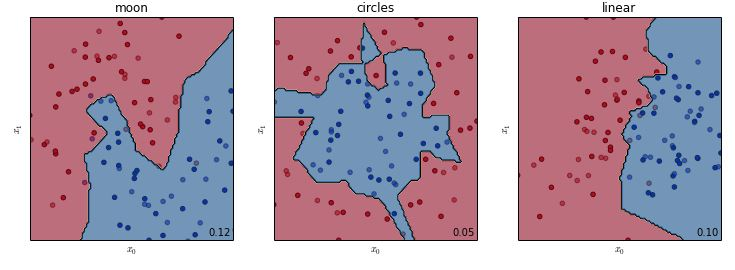
\includegraphics[width=1.1\linewidth]{sklcass/sklclass16}
	
	\end{figure}
	
\end{frame}
%======================================================%
\begin{frame}
		\frametitle{Method 3: Nearest Neighbor}
		\Large
	\textbf{Nearest Neighbours}
	\begin{itemize}
\item 	Yet Nearest Neighbor differs fundamentally from the above models in that it is a so-called non-parametric technique: the number of parameters of the model can grow infinitely as the size of the training data grows. 
\item Furthermore, it can model non-linear decision boundaries, something that is important for the first two datasets: moons and circles.
	\end{itemize}



\end{frame}

%======================================================%
\begin{frame}[fragile]
	\frametitle{Method 3: Nearest Neighbor}
	\large
	\begin{framed}
		\begin{verbatim}
	from sklearn.neighbors import KNeighborsClassifier
	
	est = KNeighborsClassifier(n_neighbors=1)
	plot_datasets(est)
		\end{verbatim}
	\end{framed}
\end{frame}

%======================================================%
\begin{frame}
	\frametitle{Method 3: Nearest Neighbor}
	\begin{figure}
		\centering
		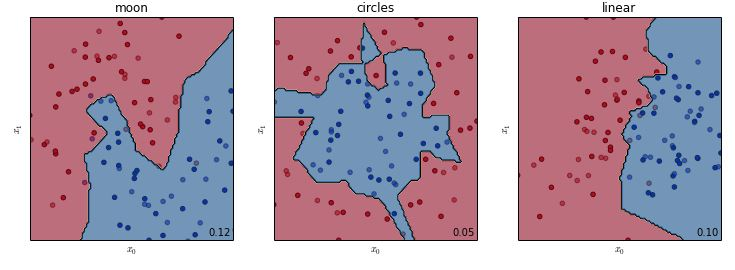
\includegraphics[width=1.1\linewidth]{sklcass/sklclass16}
		
	\end{figure}
\end{frame}
%======================================================%
\begin{frame}[fragile]
	\frametitle{Method 3: Nearest Neighbor}
	\Large
	\begin{itemize}
\item If we increase k we enforce the smoothness assumption. 
\item This can be seen by comparing the decision boundaries in the plots below where k=5 to those above where k=1.
	\end{itemize}
	{
		\large
	\begin{framed}
	\begin{verbatim}
	est = KNeighborsClassifier(n_neighbors=5)
	plot_datasets(est)
	
	\end{verbatim}
 \end{framed}
}
\end{frame}
%======================================================%
\begin{frame}
	\frametitle{Method 3: Nearest Neighbor}
\begin{figure}
\centering
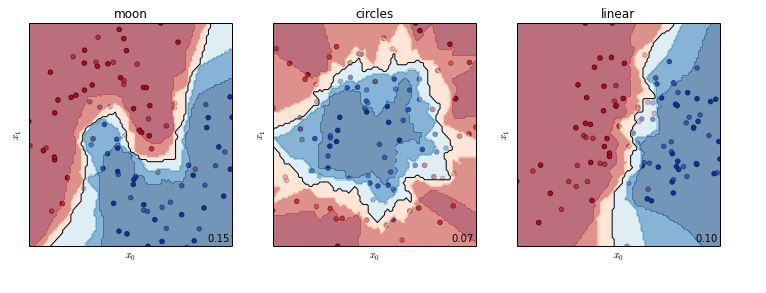
\includegraphics[width=1.1\linewidth]{sklcass/sklclass20}

\end{figure}


\end{frame}
\end{document}
